\subsection*{Problema 21}
\textbf{Enunciado:} Calcular la integral:
\begin{align*}
    I = \int \dfrac{x + \sqrt{1 - x^2}}{1 - x \sqrt{1 - x^2}} \, dx
\end{align*}

\textbf{Solución:} 
Para resolver la integral, aplicamos la sustitución trigonométrica sugerida $x = \sin\theta$, lo que implica que $dx = \cos\theta \, d\theta$. 

Además, la expresión radical se simplifica como:
\begin{align*}
    \sqrt{1 - x^2} &= \sqrt{1 - \sin^2\theta} \\
    &= \cos\theta
\end{align*}

Sustituyendo $x$, $dx$ y el radical en la integral original, obtenemos:
\begin{align*}
    I &= \int \dfrac{\sin\theta + \cos\theta}{1 - \sin\theta \cos\theta} (\cos\theta \, d\theta)
\end{align*}

Multiplicamos el numerador por $\cos\theta$:
\begin{align*}
    I &= \int \dfrac{\sin\theta\cos\theta + \cos^2\theta}{1 - \sin\theta \cos\theta} \, d\theta
\end{align*}

Multiplicamos el numerador y denominador por $2$ para facilitar el uso de identidades trigonométricas:
\begin{align*}
    I &= \int \dfrac{2\sin\theta\cos\theta + 2\cos^2\theta}{2 - 2\sin\theta \cos\theta} \, d\theta
\end{align*}

Utilizando las identidades del ángulo doble $\sin(2\theta) = 2\sin\theta\cos\theta$ y $\cos(2\theta) = 2\cos^2\theta - 1$ (es decir, $2\cos^2\theta = 1 + \cos(2\theta)$), reescribimos el integrando:
\begin{align*}
    I &= \int \dfrac{\sin(2\theta) + 1 + \cos(2\theta)}{2 - \sin(2\theta)} \, d\theta
\end{align*}

Separamos la integral en dos partes convenientes:
\begin{align*}
    I &= \int \dfrac{1}{2 - \sin(2\theta)} \, d\theta \\
    &\quad + \int \dfrac{\sin(2\theta) + \cos(2\theta)}{2 - \sin(2\theta)} \, d\theta
\end{align*}

Para la segunda integral, aplicamos sustitución directa sea $u = 2 - \sin(2\theta)$, entonces $du = -2\cos(2\theta) + 2\sin(2\theta) \, d\theta$, resolviéndose mediante logaritmos. Para la primera, empleamos la sustitución del ángulo medio $\tan(\theta) = t$. 

Tras integrar y retornar a la variable original $x$, la solución general de la integral es:
\begin{align*}
    I &= \ln\left|2 - 2x\sqrt{1-x^2}\right| + C
\end{align*}

\begin{figure}[H]
	\centering
	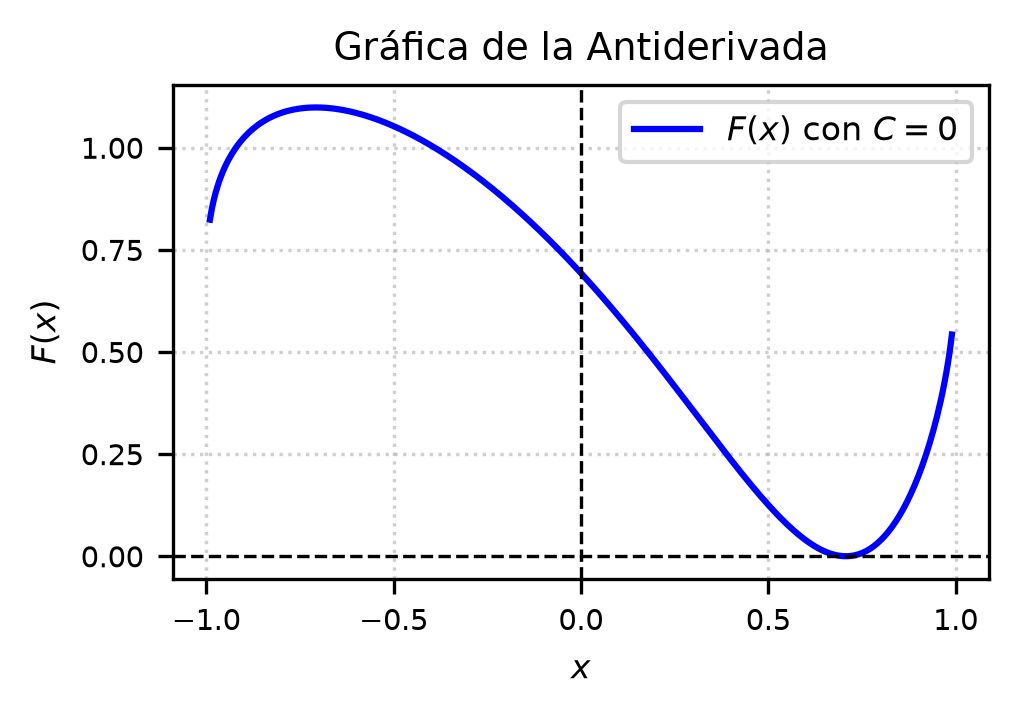
\includegraphics[width=\columnwidth]{semana_05/graficas/SEM05_P21_grafica.png}
	\caption{Representación gráfica de $f(x)$ y su antiderivada $F(x)$ evaluada para la constante de integración $C = 0$ (Problema 21).}
	\label{fig:problema21}
\end{figure}
